% This material is copyright Simon Dobnik and made available under the
% Creative Commons Attribution 4.0 International License (CC-BY-SA)
% license http://creativecommons.org/licenses/by-sa/4.0/
% 
% Email: simon.dobnik@gu.se
% Web: http://dobnik.net/simon/teaching/shared/LT2112-formling/


\documentclass{beamer}

\usepackage{graphicx,hyperref,lingmacros,qtree,fullname} 


\logo{
\includegraphics[height=0.5cm]{pics/GU-logo.pdf}} 

\newcommand{\bblue}[1]{{\usebeamercolor[fg]{frametitle}{#1}}}



\definecolor{links}{HTML}{2A1B81}
\hypersetup{colorlinks,linkcolor=,urlcolor=links}


\setbeamertemplate{footline}[frame number]


\AtBeginSection[]
{
\begin{frame}[plain]

{\huge\bblue{\insertsectionhead}}

\end{frame}
}



\newcommand{\lb}[1]{[$_{\textsf{#1}}$} 





\title[Syntax]{L2: Syntax I - POS and Phrase structure}

\author[Dobnik]{Simon Dobnik \\
Department of Philosophy, Linguistics, and Theory of Science
} 

\date{September 13, 2015}




\begin{document}



\frame[plain]{\titlepage}





\frame{

\frametitle{Outline}

\tableofcontents

}





\section{What is Syntax?}

\frame
{

\frametitle{What is Syntax?}

\begin{itemize}[<+->]

\item A formal description of \bblue{sentence structure} of natural languages.

\item Phonemes, morphemes, words, discourse units?

\item The product is a \bblue{grammar}: formal rules that approximate 
  \begin{itemize}
    \item human \bblue{linguistic intuitions/competence},
    \item or valid strings in a language.
  \end{itemize}

\item Rules must be abstracted from linguistic evidence: human \bblue{performance}.

\item Natural language syntax and syntax of programming languages

\end{itemize}

}





\frame{

\frametitle{Some syntactic properties of natural languages}


\begin{itemize}[<+->]

\item \bblue{Infinite number of sentences} \\ Alex said that Lydia thought that George wondered\ldots

\item \bblue{Units of sentences are hierarchically organised into larger units } \\ spider on the wall, big spider on the wall, the big spider on the wall, the very big green vicious spider on the wall

\item \bblue{Dependencies between units} \\ George saw \underline{\hspace{0.5cm}}. \\ Lydia enjoy\underline{\hspace{0.5cm}} playing Jawbreaker.

\item \bblue{Similar kinds of sentences where units appear ``displaced''.} \\
Lydia bought some violets. \\ The violets were bought by Lydia.


\end{itemize}

}





\frame{

\frametitle{Some history}

\begin{itemize}

\item Writing grammars of natural languages (of any kind) has a long tradition.

\item Attempts of formal accounts of grammar: \href{http://en.wikipedia.org/wiki/P\%C4\%81\%E1\%B9\%87ini}{P\={a}\d{n}ini}, 4th century BC.

\item Generative Grammar: Noam Chomsky. Syntactic Structures. 1957. 
\end{itemize}

}





\frame{

\frametitle{Main principles of Generative Grammar}

\begin{enumerate}

\item Grammars should be formal.

\pause

\item  A theory of human linguistic ability. \\
	\begin{itemize}[<+->]
		\item Universal grammar (UG): innate to human beings.
		\item Variations between languages are parameters set during language acquisition.
		\item Syntactic processes are central in human language production/understanding and reasoning.
		\end{itemize}

\end{enumerate}

\pause

\bigskip

\bblue{1} accepted widely today; \bblue{2} has been criticised.


}





\section{Formal grammars}

\frame{

\frametitle{Formal grammar}

A formal grammar consists of:

\begin{itemize}

\item a finite set of terminal symbols: a, b, $\epsilon$ (empty string);

\item a finite set of non-terminal symbols: A, B;

\item a finite set of production rules: A $\rightarrow$ aB, B $\rightarrow$ b, aB $\rightarrow$ A;

\item a start symbol: S $\rightarrow$ AB.

\end{itemize}

\pause

\bigskip

\bblue{Derivation:} start with S and apply the sequence of rules by replacing symbols on the LHS with those on the RHS; stop when all symbols are non-terminal.


}





\frame{

\frametitle{A comparison of formal grammars}

Increasing the power of production rules generates different kinds of formal grammars\ldots

\bigskip

\begin{tabular}{l l l}
\hline
\bblue{Grammar} & \bblue{Language} & \bblue{Production rules allowed} \\
\hline
Type-0 & Recursively enumerable & $\alpha$ $\rightarrow$ $\beta$ (unrestricted) \\
Type-1 & Context sensitive & $\alpha$A$\beta$ $\rightarrow$ $\alpha \gamma \beta$ \\
Type 2 & Context-free & A $\rightarrow$ $\gamma$ \\
Type-3 & Regular & A $\rightarrow$ a and A $\rightarrow$ aB
\end{tabular}

\bigskip

\bblue{A:} non-terminal symbol; \bblue{a:} terminal symbol; \bblue{$\alpha, \beta, \gamma$:} terminal or non-terminal symbols
 

}





\frame{

\frametitle{Chomsky hierarchy}

\begin{center}
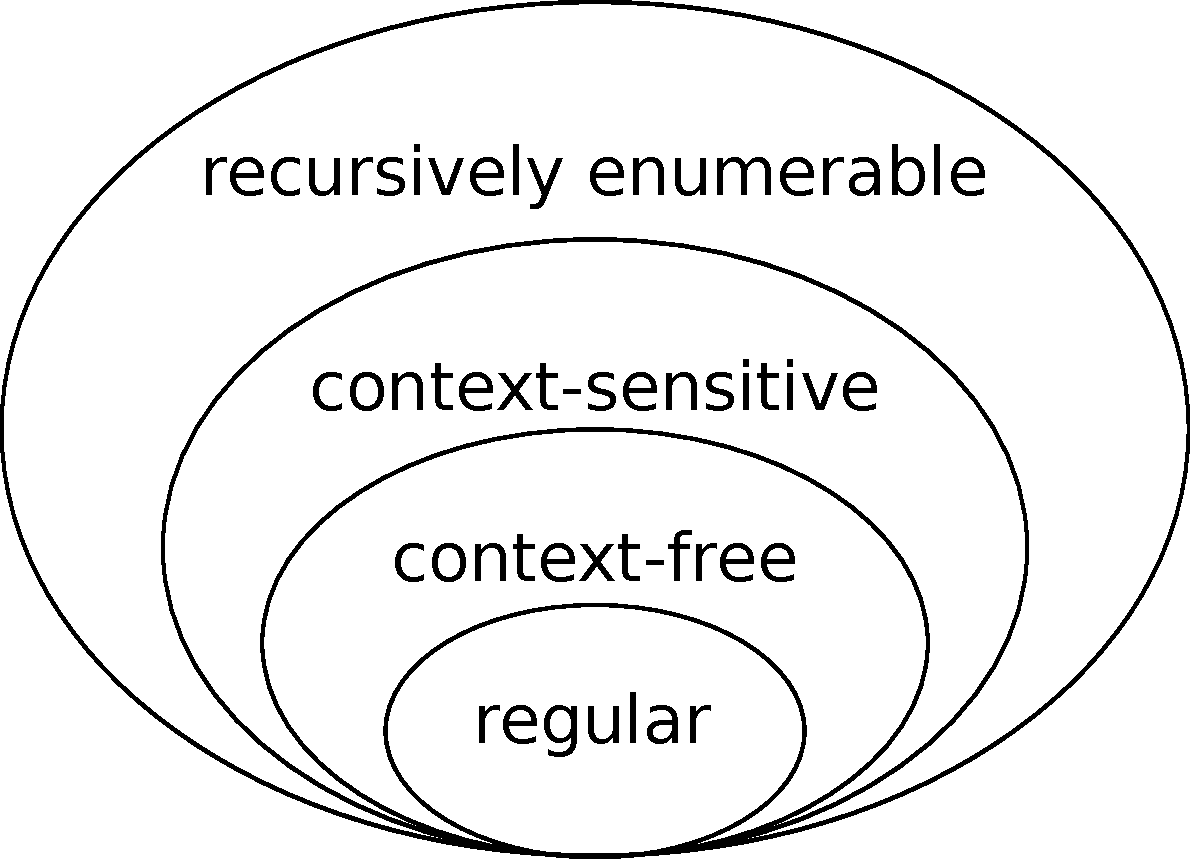
\includegraphics[scale=0.33]{./pics/Chomsky-hierarchy.pdf}
\end{center}

From \href{http://en.wikipedia.org/wiki/Chomsky_hierarchy}{Wikipedia}

}





\section{Terminal symbols: words}


\frame{

\frametitle{Terminal symbols: Parts of speech (POS)}

How can we tell that there are different classes of words?

\pause

\bigskip

\bblue{Semantic criteria:} ``a noun is a place a person or a thing''.

\pause

\eenumsentence{
\item The \bblue{destruction} of the city was inevitable. \item They frequently \bblue{phone} each other. \item They \bblue{quanded} the \bblue{medin} \bblue{exbontigly}. }
\pause

\bigskip

Not very useful.

}





\frame{

\frametitle{Distributional criteria}


\pause

\bblue{Morphological distribution:} what kind of affixes a word can take

\begin{itemize}

\item \bblue{Inflectional:} big, bigg\textbf{-er}, big\textbf{-est} (A), *friend\textbf{-est} ($\neg$A)

\pause

\item \bblue{Derivational:} person (N), person\textbf{-al} (A), read (?), *read\textbf{al}

\end{itemize}

\pause

\bigskip

\bblue{Syntactic distribution:} what kind of words appear around that word


\eenumsentence{
\item The \ldots became popular in the second half of the 19th century: (\href{http://en.wikipedia.org/wiki/History_of_photography}{photography}, $\neg$to).

\pause

\item Peter was eager to \ldots: (leave, $\neg$green).

}

}





\frame{

\frametitle{Types of POS}

\bblue{Open and closed class} 

\eenumsentence{
  \item I \bblue{googled} their name: V.
  \item *The chair is to the \bblue{nearleft} of the table: P or Adv.
}

\pause \bigskip

\bblue{Lexical and functional categories:} semantic content \bblue{vs} grammatical function

\enumsentence{
\underline{Many/D} managers/N \underline{could/Mod} \underline{be/Aux} sacked/V \underline{by/P} \underline{the/D} board/N.
}


}





\frame{

\frametitle[allowframebreaks]{How many classes?}

It depends on the language and the grammar you want to build.

\pause \bigskip

\begin{itemize}

\item \bblue{Nouns (N):} John, apple, grass \\
proper vs. common, countable vs. mass

\item \bblue{Verbs (V):} rains, kisses, give \\
intransitive, transitive, and ditransitive

\item \bblue{Adjectives (A):} new, surprising 

\item \bblue{Adverbs (Adv):} quickly, honestly

\item \bblue{Pronouns and anaphora (N or Pron):} he, her, which, itself

\item \bblue{Determiners (D):} a, an, the, this, every, none, no, three, your, which

\item \bblue{Prepositions (P):} in, on, at

\item \bblue{Complenetisers (C):} that, for, if, whether

\item \bblue{Conjunctions (Conj):} and, or, nor, either, neither

\item \bblue{Negation (Neg):} not, non

\item \bblue{Auxiliaries (Aux):} is, do, have, to

\item \bblue{Modal verbs (Mod):} will, would, shall, should, can, could

\end{itemize}

}





\frame{

\frametitle{The Penn Treebank set of POS}

\href{http://www.cis.upenn.edu/~treebank/}{http://www.cis.upenn.edu/$\sim$treebank/}

\pause

\begin{itemize}

\item Finer distinctions: \\
  \begin{itemize}
  \item VB: Verb, base form: \bblue{take}
  \item VBD: Verb, past tense: \bblue{took}
  \item VBG: Verb, gerund or present participle: \bblue{taking}
  \item VBN: Verb, past participle: \bblue{taken}
  \item VBP: Verb, non-3rd person singular present: \bblue{take}
  \item VBZ: Verb, 3rd person singular present: \bblue{takes}
  \end{itemize}

\item \pause Subcategories are typically represented as \bblue{features} in theoretical grammars.

\item \pause \href{https://www.ling.upenn.edu/courses/Fall_2003/ling001/penn_treebank_pos.html}{Full list}

\item \pause \href{ftp://ftp.cis.upenn.edu/pub/treebank/doc/tagguide.ps.gz}{Tagging guide}

\end{itemize}

}





\frame{

\frametitle{Why do POSs matter for NLP?}

The POS of a word (tagging) tells us 

\begin{itemize}

\item how the word fits with other words to make a sentence (parsing);

\item gives us some semantic information.

\end{itemize}

\bigskip

\eenumsentence{
  \item Flying/A planes/N can/Mod be/Aux dangerous/A.
  \item Flying/V planes/N can/Mod be/Aux dangerous/A.
}

}





\frame{

\frametitle{POS tagging and context}

The most likely POS for an ambiguous word can be resolved from the context.

\bigskip

\eenumsentence{
  \item They/N can/Aux fish/N in/P the/D lake/N.
  \item They/N can/V fish/N at/P the/D factory/N.
}

}





\section{Non-terminal symbols: phrases}

\subsection{Tests for constituents}

\frame{

\frametitle{Constituent/phrase structure}

Words associate with certain other words and form units.

\bigskip

\eenumsentence{
\item Peter kicked [the cat].
\item *Peter [kicked the] cat.
}

\pause

\eenumsentence{
  \item {}[Jane] loves [his new book on syntax].
  \item {}[Bill] hates [his annoying colleague from work].
}



}





\frame{

\frametitle{Tests for constituency: replacement}


Similar units can be replaced.

\eenumsentence{
  \item {}[The man with an umbrella] [read] [the book with the green cover].
  \item {}[He] [wrote] [it].
  \item {}[They] [ran].
}

}





\frame{

\frametitle{Tests for constituency: sentence fragment}


\eenumsentence{
  \item What did Peter do yesterday?
  \item Read the book with the green cover.
  \item *Read the.
}
}





\frame{

\frametitle{Tests for constituency: coordination}

Only similar items can be conjoined.

\bigskip

\eenumsentence{
  \item Peter [[read the book] and [washed the dishes yesterday]].
  \item Peter [[read the book] and [ran]].
  \item {}[[Peter] and [his wife]] [read the book].
}
}





\frame{

\frametitle{Tests for constituency: displacement}


\eenumsentence{
  \item John looked up a word.
  \item John looked up a tree.
  \item The word/the tree, John looked up.
  \item *Up the word, John looked.
  \item Up the tree, John looked.
}


}





\subsection{A CFG fragment of English}

\frame{

\frametitle{A fragment of English: some CFG rules}

CFG rules can be of the following form: A $\rightarrow$ $\gamma$+

\pause

\bigskip

\begin{enumerate}[<+->]

\item Alex, tree, books: NP $\rightarrow$ N

\item the cat, a cat, cats: NP $\rightarrow$ (D) N

\item the big cat, the big cat with blue ears: \\ NP $\rightarrow$ (D) (AP+) N (PP+), PP $\rightarrow$ P NP

\item the very big cat, the very big fluffy cat: \\AP $\rightarrow$ (AdvP) A

\item very quickly: AdvP $\rightarrow$ (AdvP) Adv

\end{enumerate}

}





\frame{

\frametitle{More CFG rules}

The verb phrase\ldots

\pause

\begin{enumerate}

 \item[6.] Alex left. Alex deliberately always left quietly early.\\
 VP $\rightarrow$ (AdvP+) V (AdvP+)
 
\pause

 \item[7.]  Alex suddenly kissed Lydia.\\ Alex gave Lydia a present yesterday.\\
 VP $\rightarrow$ (AdvP+) V (NP) (NP) (AdvP+)

\pause
 
 \item[8.] Alex gave a present quietly to Lydia in the garden yesterday.\\
 VP $\rightarrow$ (AdvP+) V (NP) (NP) (AdvP+) (PP+) (AdvP+)

\end{enumerate}

}





\frame{

\frametitle{And finally\ldots}

\begin{itemize}

\item[9.] Alex left. Alex gave a present\ldots \\
S $\rightarrow$ NP VP

\pause

\item[10.] Alex has scared the ducks. Alex may leave. \\
TP $\rightarrow$ NP (T) VP 

\pause

\item[11.] Lydia said that Alex scared the ducks.\\
Lydia asked George if Alex scared the ducks. \\
CP $\rightarrow$ (C) TP \\
VP $\rightarrow$ (AdvP+) V (NP) (\{NP/CP\}) (AdvP+) (PP+) (AdvP+)

\end{itemize}

}





\section{Phrase structure}

\subsection{Representing phrase structure}

\frame{

\frametitle{Representing phrase structure}

\bblue{Bracketing} 

{\footnotesize
\lb{TP} \lb{NP} \lb{N} Alex ] ] \lb{VP} \lb{V} gave ] \lb{NP} \lb{N} Lydia ] ] \lb{NP} \lb{D} a ] \lb{N} present ] ] \lb{AdvP} \lb{Adv} yesterday ] ] ] ]
}

\bigskip

\pause

\bblue{Trees} 

{\footnotesize
\Tree [.TP [.NP [.N Alex ] ] [.VP [.V gave ] [.NP [.N Lydia ] ] [.NP [.D a ] [.N present ] ] [.AdvP [.Adv yesterday ] ] ] ]
}

}





\frame{

\frametitle{Properties of CFG}

\begin{enumerate}[<+->]

\item Context free: a phrase can be applied independently of its context (no context on the LHS of rules). 

\item A phrase has its internal structure (RHS of rules).

\item Phrases cannot be discontinued or overlap each other.

\item They are either disjoint or contain one another.

\item \bblue{Recursive} application of rules is allowed: XP $\rightarrow$ Y XP

\end{enumerate}


}





\frame{

\frametitle{Properties that are not part of the CFG}

and are required to model language:

\pause

\begin{enumerate}

\item Phrases have \bblue{heads} (terminal symbols) that determine the category of a phrase.

\pause

\item Heads are modified by other phrases (\bblue{modifiers}).

\pause

\item Selectional restrictions of constituents:\\
	\begin{itemize}
		\item \bblue{Agreement:} Alex/They likes/like butterflies.
		\item \bblue{Sub-categorisation:} Alex liked *(the park).
	\end{itemize}

\pause

\item \bblue{``Random'' laws of human language:} \\Sentences must have subjects: It rains.

\pause

\item \bblue{Sentence meaning:} The tree climbed up Alex.

\end{enumerate}

}





\frame{

\frametitle{Some examples CFG cannot handle}

\bblue{Agreement is context sensitive}

\eenumsentence{
  \item John sleeps.
  \item They sleep.
}

\pause

\bblue{Discontinuous and overlapping phrases}

\eenumsentence{
  \item John bought and Mary sold a car.
  \item A man arrived who looked very strange (discontinued).
  \item I read what was on the reading list (overlapping `what').
}

\pause

\bigskip

Sufficient to describe most human languages. \\(NB: \href{http://en.wikipedia.org/wiki/Swiss_German}{Swiss German}, \href{http://en.wikipedia.org/wiki/Bambara_language}{Bambara})

}



























































\subsection{Syntactic ambiguity}

\frame{

\frametitle{Syntactic ambiguity}

\footnotesize


\enumsentence{\lb{TP} \lb{NP} \lb{N} She] ] \lb{VP} \lb{V} saw ] \lb{NP} \lb{D} a ] \lb{NP} \lb{N} man] ] ] \lb{PP} \lb{P} with ] \lb{NP} a \lb{N} telescope ] ] ] ] ] }


\Tree  [.TP [.NP [.N She ]  ] [.VP [.V saw ] [.NP [.D a ] [.NP [.N man ] ] ] [.PP [.P with ] [.NP a [.N telescope ] ] ] ] ]

}





\frame{

\footnotesize


\enumsentence{\lb{TP} \lb{NP} \lb{N} She] ] \lb{VP} \lb{V} saw ] \lb{NP} \lb{D} a ] \lb{NP} \lb{N} man] ] \lb{PP} \lb{P} with ] \lb{NP} a \lb{N} telescope ] ] ] ] ] ] }

\Tree  [.TP [.NP [.N She ]  ] [.VP [.V saw ] [.NP [.D a ] [.NP [.N man ] ]  [.PP [.P with ] [.NP a [.N telescope ] ] ] ] ] ]

}





\frame{

\frametitle{Further reading}

\cite{Allen:1995aa} Chapter 2 (Linguistic background: an outline of English syntax)

\bigskip

\cite{Jurafsky:2009uq} Chapters 5.1: (Mostly) English word classes, 5.2 Tag-sets for English, Chapter 12: Formal grammars of English and Chapter 16: Language and Complexity

\bigskip

\cite{Carnie:2007aa} Chapters 2 (Parts of speech) and 3 (Constituency, trees and rules).

\bigskip

\cite{Tallerman:2011aa} 
\bigskip

\cite{Pinker:1995aa} Chapters 4 to 7.

}





\begin{frame}[allowframebreaks]{References}

\small


\bibliographystyle{fullname}
\bibliography{bibliography}


\end{frame}





\end{document}




